\documentclass[a4paper,12pt]{article}
\usepackage[english]{babel}
\usepackage[utf8]{inputenc}
\usepackage{amsfonts}
\usepackage{indentfirst}
\usepackage[T1]{fontenc}
\usepackage{amsmath}
\usepackage{hyperref}
\usepackage{graphicx}
\usepackage{subfig}
\usepackage[export]{adjustbox}

\textwidth\paperwidth
\advance\textwidth -45mm
\oddsidemargin 18mm
\advance\oddsidemargin -18mm
\evensidemargin 18mm
\advance\evensidemargin -18mm
\topmargin -30mm
\advance\topmargin 17mm
\setlength\textheight{45\baselineskip}
\addtolength\textheight{\topskip}
\marginparwidth 15mm


\title{
  \textbf{Human Recognition by Biometric Methods}\\
  \bigskip
  \textbf{Face classification}\\  
  \bigskip
}
\author{Mikołaj Małkiński}
\date{12 April 2018}

\begin{document}

\maketitle

\section{Description of the assignment}

The goal of this task was to design, implement and train a Convolutional Neural Network model for recognizing faces of (four) Polish rappers. Several different architectures were analysed, where the difference was mainly in the choice of base models: VGG16, ResNet50 and InceptionV3.
\par
The original dataset was split into two parts: train (1600 images of each class) and validation (400 images of each class). The models are trained only on the train dataset and their accuracies are evaluated on the validation dataset.
\par
The models are resizing the images before processing, so data of arbitrary size can be used. This procedure is done using ImageDataGenerator - a tool provided by Keras, which feeds data from directory into the model. Furthermore, it offers several data augmentation functionalities, which will be discussed later.
\par
The project conists of following scripts:
\begin{itemize}
\item $evaluate$ - evaluates model accuracy and loss on specified dataset,
\item $predict$ - predicts a class of specified image,
\item $reproduce\_results$ - creates plots shown in the report,
\item $train$ - trains given model on specified dataset.
\end{itemize}

\section{Overview of used models}
Network architectures were created using already existing solutions, with modified top layers. Figure \ref{fig:custom_top_models} presents which layers were added on top of base-line architectures, which were initialized with weights trained on the ImageNet dataset. During training, mostly the top layers were trained, with exception  of one solution which used fine-tuning, which will be discussed later.
\begin{figure}[!h]
\centering
\begin{tabular}{ccc}
	\subfloat[VGG16]{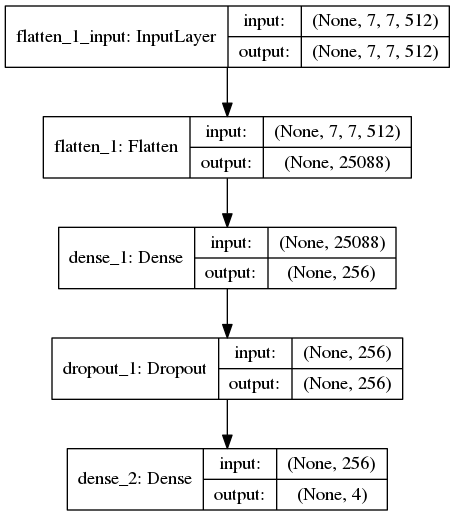
\includegraphics[width = 0.3\textwidth]{plots/vgg16_top_model_plot.png}} &
	\subfloat[ResNet50]{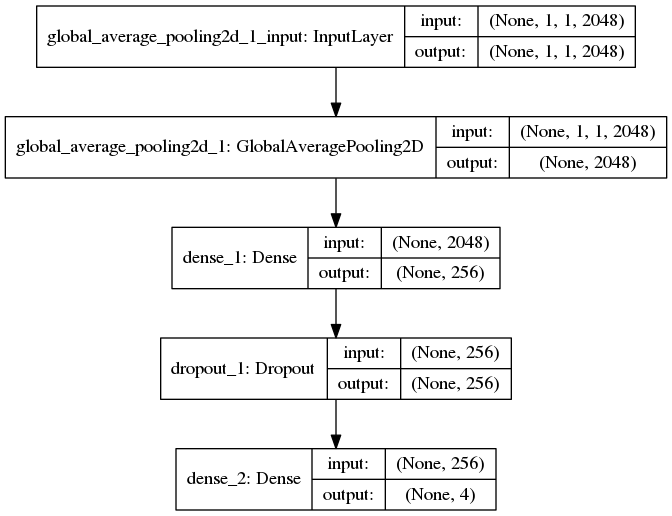
\includegraphics[width = 0.3\textwidth]{plots/resnet50_top_model_plot.png}} &
	\subfloat[InceptionV3]{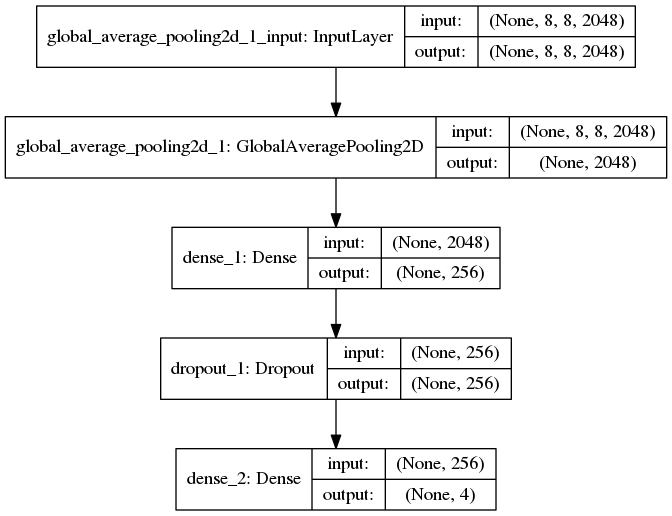
\includegraphics[width = 0.3\textwidth]{plots/inceptionv3_top_model_plot.png}}
\end{tabular}
\caption{Custom top models}
\label{fig:custom_top_models}
\end{figure}

There was a noticeable difference between mentioned architectures. Figure \ref{fig:base_model_compare} presents the training process. Networks created with the use of VGG16 and InceptionV3 gave satisfying results, which are presented in the Figure \ref{fig:results}. However, ResNet50 seems to be way behind the competition.
\begin{figure}[!h]
\centering
\begin{tabular}{cc}
	\subfloat{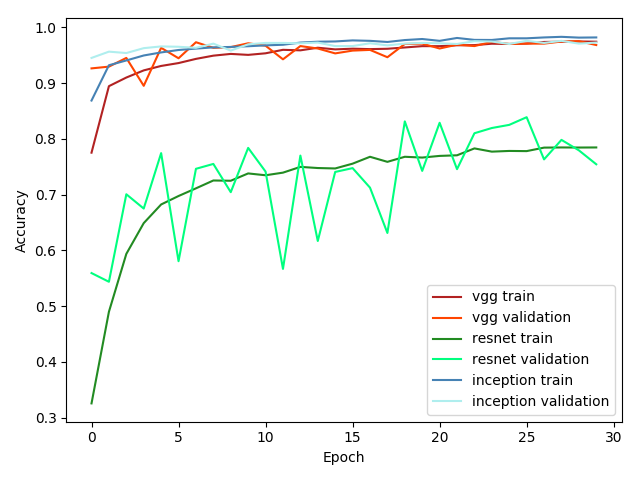
\includegraphics[width = 0.4\textwidth]{plots/base_model_compare_acc.png}} &
	\subfloat{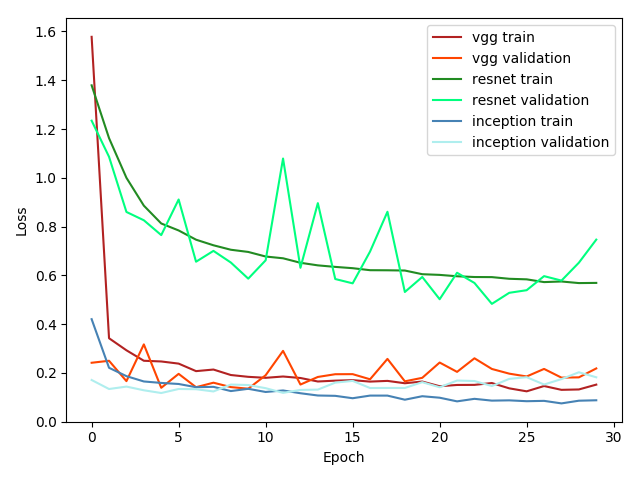
\includegraphics[width = 0.4\textwidth]{plots/base_model_compare_loss.png}} \\
\end{tabular}
\caption{Performance of VGG16, ResNet50 and InceptionV3 with custom top models}
\label{fig:base_model_compare}
\end{figure}

\begin{figure}[!h]
\centering
\begin{tabular}{cccc}
	& VGG16 & ResNet50 & InceptionV3 \\
	accuracy & 0.9681 & 0.8231 & 0.9506 \\
	loss & 0.2902 & 0.5178 & 0.7757 \\
\end{tabular}
\caption{Results obtained on validation set}
\label{fig:results}
\end{figure}

\section{Data augmentation}
One possibility to improve the accuracy of network, is to use data augmentation. Keras provides a utility called ImageDataGenerator, which is quite convenient for this task. It's options are well described in the documentation. Figure \ref{fig:vgg16_da_compare} presents the effect of applying data augmentation for VGG16 architecture. Unfortunately, it didn't give satisfactory results, probably because the dataset seems to be already influenced by some kind of data augmentation. The numerical results are shown in the Figure \ref{fig:results_da}.
\begin{figure}[!h]
\centering
\begin{tabular}{cc}
	\subfloat{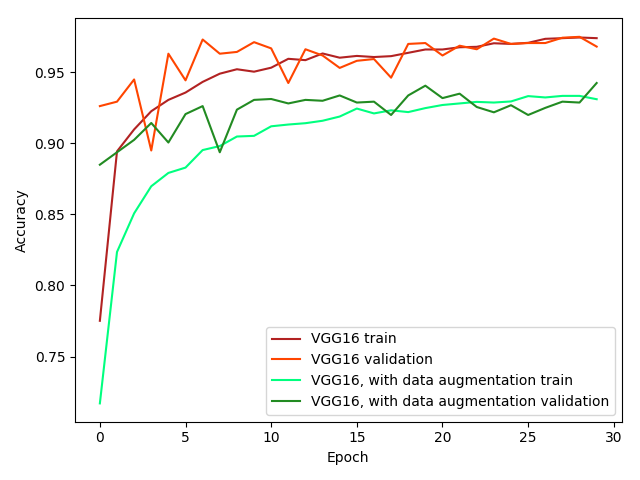
\includegraphics[width = 0.4\textwidth]{plots/vgg16_da_compare_acc.png}} &
	\subfloat{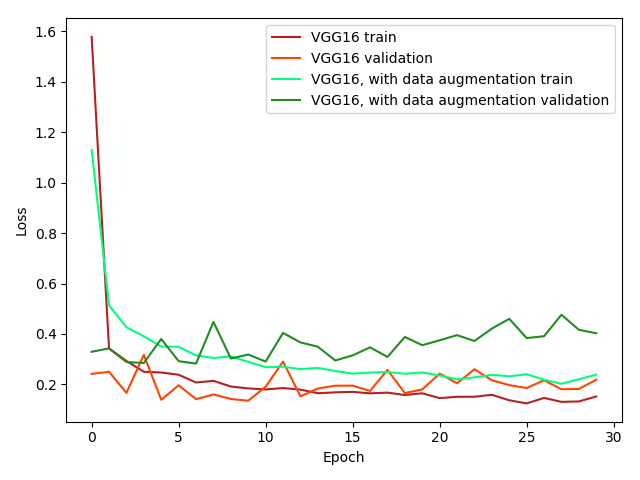
\includegraphics[width = 0.4\textwidth]{plots/vgg16_da_compare_loss.png}} \\
\end{tabular}
\caption{Influence of data augmentation on VGG16}
\label{fig:vgg16_da_compare}
\end{figure}

\begin{figure}[!h]
\centering
\begin{tabular}{ccc}
	& Original dataset & With data augmentation \\
	accuracy & 0.9681 & 0.9425 \\
	loss & 0.2902 & 0.4028 \\
\end{tabular}
\caption{Results of VGG16}
\label{fig:results_da}
\end{figure}

\section{Fine tuning}
After training the top layers, it is often desirable to freeze them, and proceed with training several layers from the base architecture. This technique is called fine-tuning and can yield noticeable improvements. In this case, using VGG16 as base model, it gave improvement of more than 1\%, which is a good result considering the fact, that plain base model had already accuracy of almost 97\%. The training process is presented in the Figure \ref{fig:vgg16_ft_compare}. Observer that the fine-tuned version has big accuracy starting from the first epochs, because the top layers were already trained. Numerical results computed on validation and training sets are shown in Figures \ref{fig:results_ft_val} and \ref{fig:results_ft_train}.
\begin{figure}[!h]
\centering
\begin{tabular}{cc}
	\subfloat{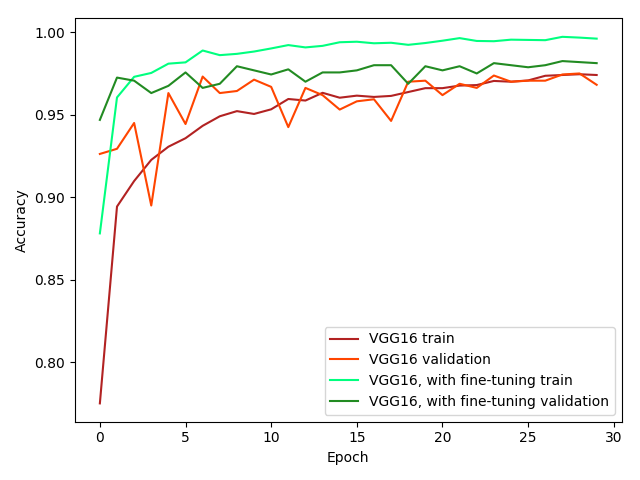
\includegraphics[width = 0.4\textwidth]{plots/vgg16_ft_compare_acc.png}} &
	\subfloat{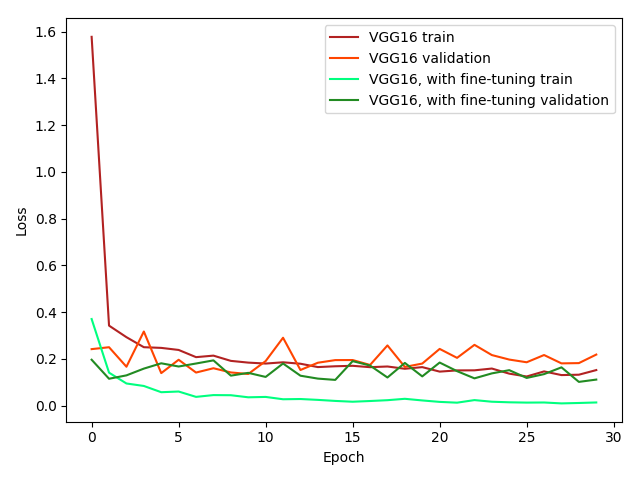
\includegraphics[width = 0.4\textwidth]{plots/vgg16_ft_compare_loss.png}} \\
\end{tabular}
\caption{Influence of fine-tuning on VGG16}
\label{fig:vgg16_ft_compare}
\end{figure}

\begin{figure}[!h]
\centering
\begin{tabular}{ccc}
	& Only top model trained & Fine-tuning \\
	accuracy & 0.9681 & 0.98125 \\
	loss & 0.2902 & 0.11157 \\
\end{tabular}
\caption{Results of VGG16 on validation set}
\label{fig:results_ft_val}
\end{figure}
\begin{figure}[!h]
\centering
\begin{tabular}{ccc}
	& Only top model trained & Fine-tuning \\
	accuracy & 0.9858 & 0.9992 \\
	loss & 0.0926 & 0.0049 \\
\end{tabular}
\caption{Results of VGG16 on training set}
\label{fig:results_ft_train}
\end{figure}

\section{Hyperparameters}

\subsection{Batch size}
Batch size is one of the hyperparameters which can influence the network accuracy. During experiments, two batch sizes were analysed: 16 and 32. Unfortunately, starting from 64, the batch of images wasn't able to bewas too big to fit it into GPU memory. In the Figure \ref{fig:vgg16_bs_compare} the influence of mentioned batch sizes are shown. It can be noticed, that larger batch size gave slightly better results, but the difference isn't huge.
\begin{figure}[!h]
\centering
\begin{tabular}{cc}
	\subfloat{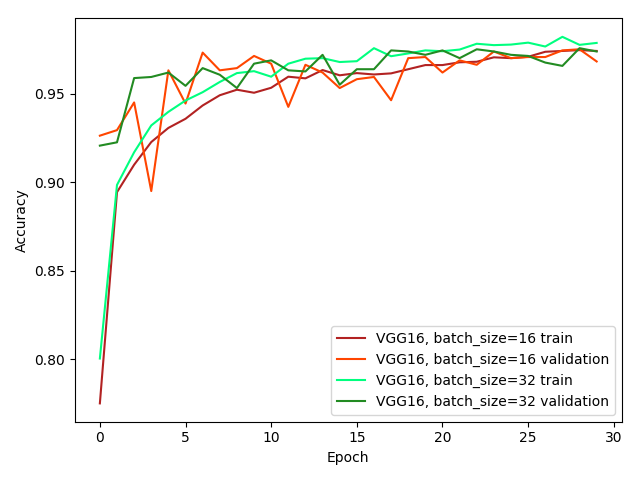
\includegraphics[width = 0.4\textwidth]{plots/vgg16_bs_compare_acc.png}} &
	\subfloat{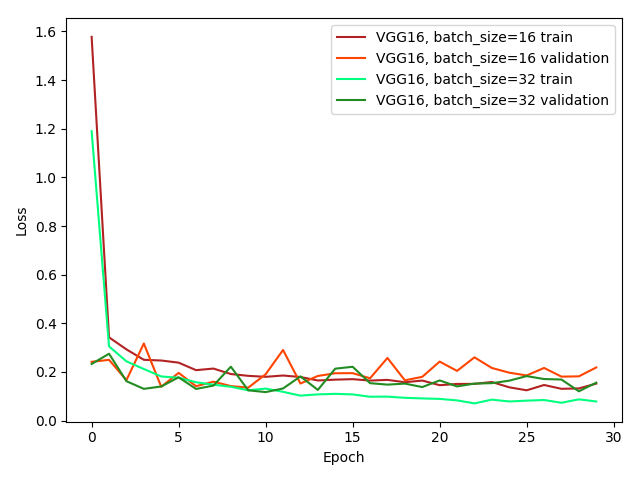
\includegraphics[width = 0.4\textwidth]{plots/vgg16_bs_compare_loss.png}} \\
\end{tabular}
\caption{Performance of VGG16 using different batch size}
\label{fig:vgg16_bs_compare}
\end{figure}

\subsection{Optimizers}
Optimizers are another kind of hyperparameters which can influence the time needed to train the network as well as it's accuracy. Figure \ref{fig:vgg16_rms_adam_compare} presents results obtained using default RMSprop and Adam optimizers. The results are rather similar. However, the choice of learning rate can be crucial for reasonable convergence time and accuracy. In the Figure \ref{fig:vgg16_rms_big_lr_compare} a deteriorating impact of RMSprop optimizer with too big learning rate is presented. On the other hand, Figure \ref{fig:vgg16_rms_small_lr_compare} highlights how slow a network converges, when the learning rate is too low. During experiments, it was found out that default optimizer values bundled into Keras give satisfactory results.
\begin{figure}[!h]
\centering
\begin{tabular}{cc}
	\subfloat{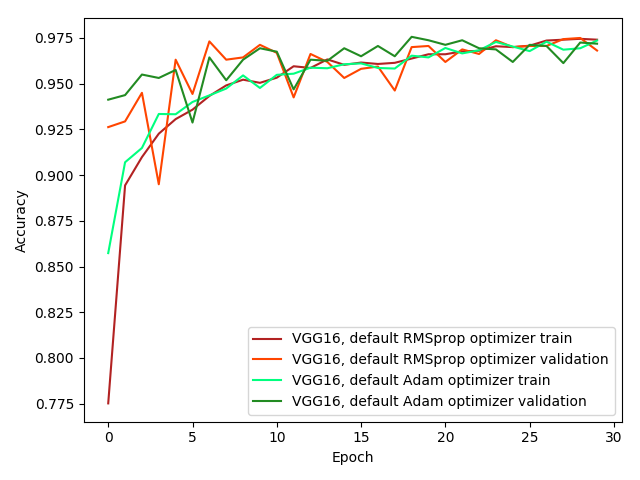
\includegraphics[width = 0.4\textwidth]{plots/vgg16_rms_adam_compare_acc.png}} &
	\subfloat{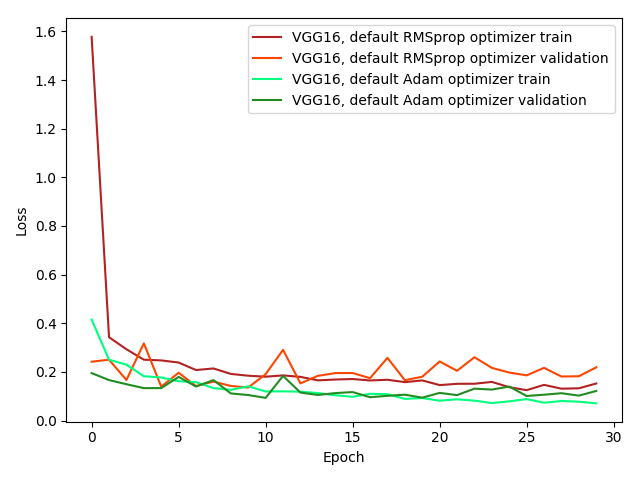
\includegraphics[width = 0.4\textwidth]{plots/vgg16_rms_adam_compare_loss.png}} \\
\end{tabular}
\caption{Default RMSprop and Adam optimizers for VGG16}
\label{fig:vgg16_rms_adam_compare}
\end{figure}

\begin{figure}[!h]
\centering
\begin{tabular}{cc}
	\subfloat{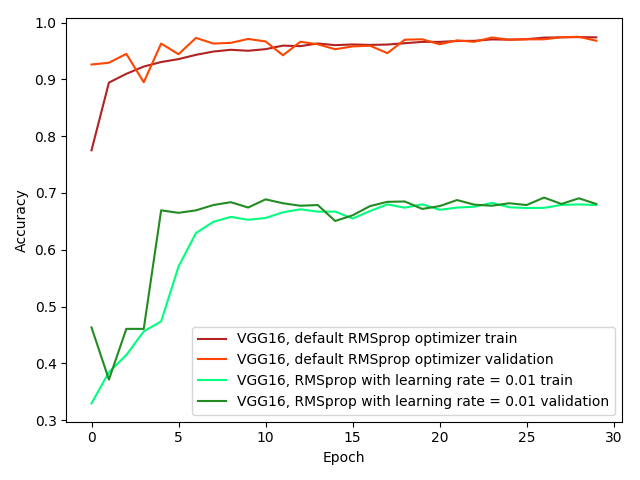
\includegraphics[width = 0.4\textwidth]{plots/vgg16_rms_big_lr_compare_acc.png}} &
	\subfloat{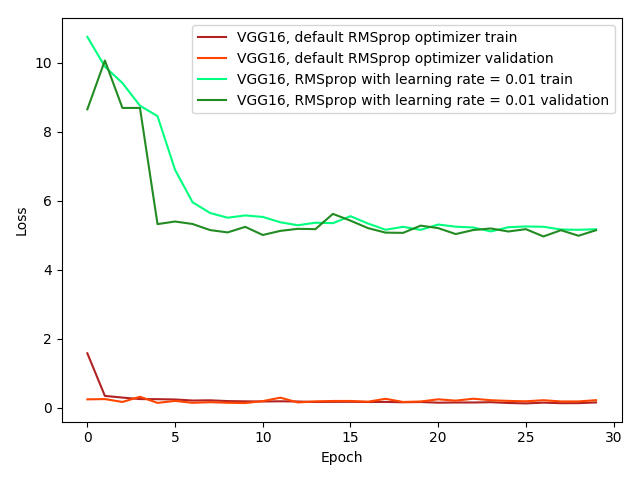
\includegraphics[width = 0.4\textwidth]{plots/vgg16_rms_big_lr_compare_loss.png}} \\
\end{tabular}
\caption{Influence of RMSprop optimizer with learning rate = 0.01 on VGG16}
\label{fig:vgg16_rms_big_lr_compare}
\end{figure}

\begin{figure}[!h]
\centering
\begin{tabular}{cc}
	\subfloat{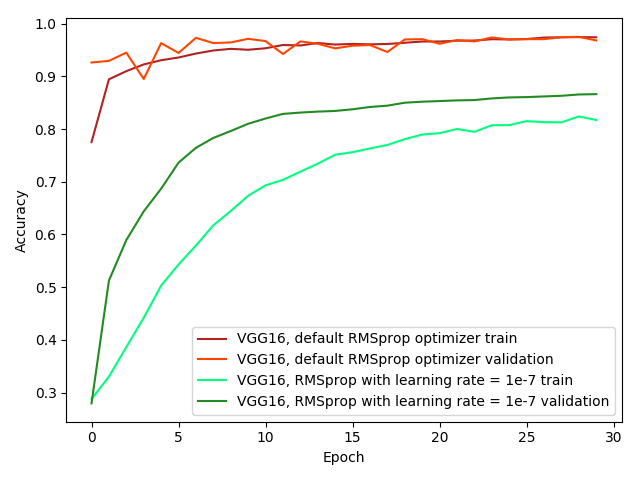
\includegraphics[width = 0.4\textwidth]{plots/vgg16_rms_small_lr_compare_acc.png}} &
	\subfloat{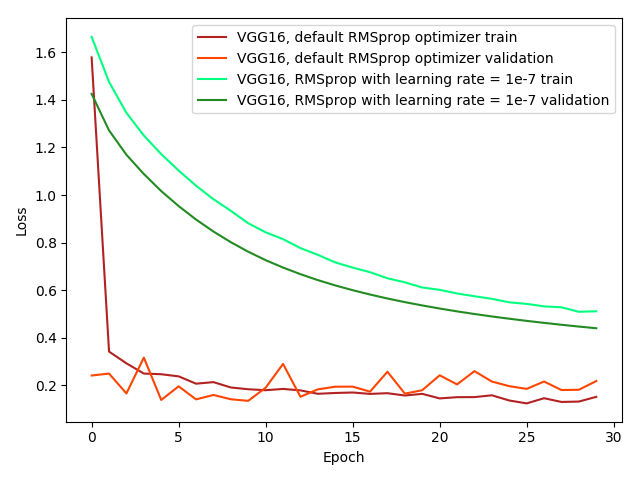
\includegraphics[width = 0.4\textwidth]{plots/vgg16_rms_small_lr_compare_loss.png}} \\
\end{tabular}
\caption{Influence of RMSprop optimizer with learning rate = 1e-7 on VGG16}
\label{fig:vgg16_rms_small_lr_compare}
\end{figure}

\subsection{Dropout}
To prevent a strong network from overfitting, dropout can be applied. The Figure \ref{fig:resnet50_dropout_compare} shows the effect of including dropout layer, with value = 20\%, into top model put on top of ResNet50 architecture. In this case, including dropout layer only reduced the accuracy. Finally in the Figure \ref{fig:resnet50_100e_da02_compare}, mentioned architecture with dropout is analysed on larger amount of epochs.

\begin{figure}[!h]
\centering
\begin{tabular}{cc}
	\subfloat{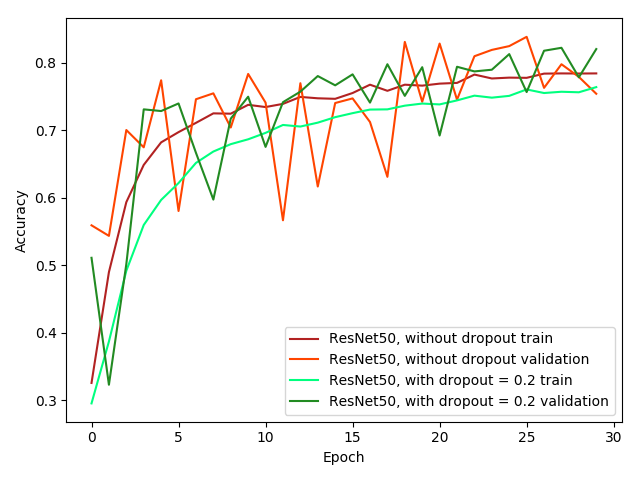
\includegraphics[width = 0.4\textwidth]{plots/resnet50_dropout_compare_acc.png}} &
	\subfloat{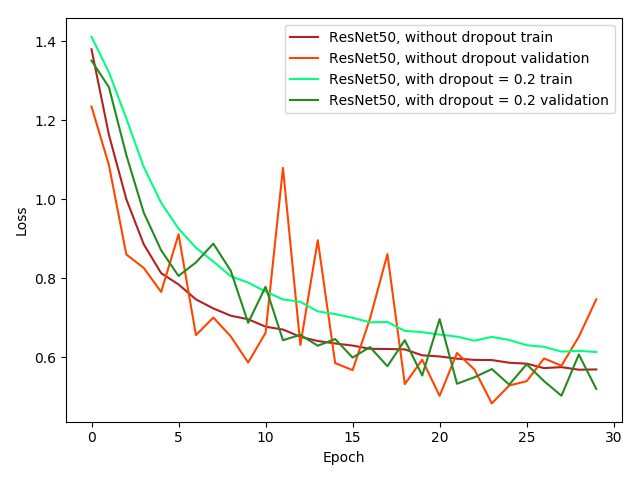
\includegraphics[width = 0.4\textwidth]{plots/resnet50_dropout_compare_loss.png}} \\
\end{tabular}
\caption{Performance of ResNet50 with dropout in top model}
\label{fig:resnet50_dropout_compare}
\end{figure}
\begin{figure}[!h]
\centering
\begin{tabular}{cc}
	\subfloat{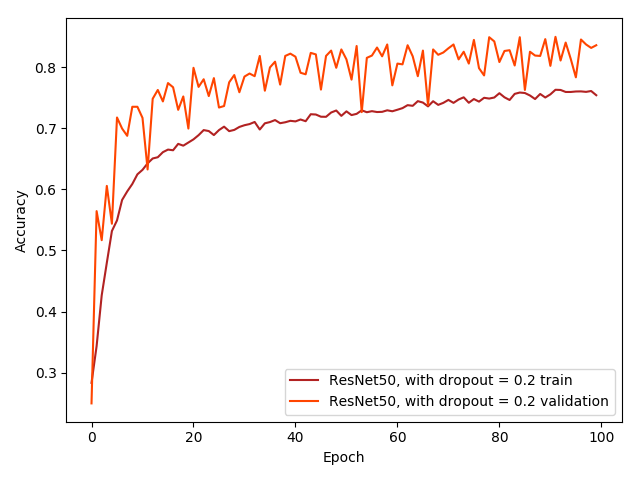
\includegraphics[width = 0.4\textwidth]{plots/resnet50_100e_da02_acc.png}} &
	\subfloat{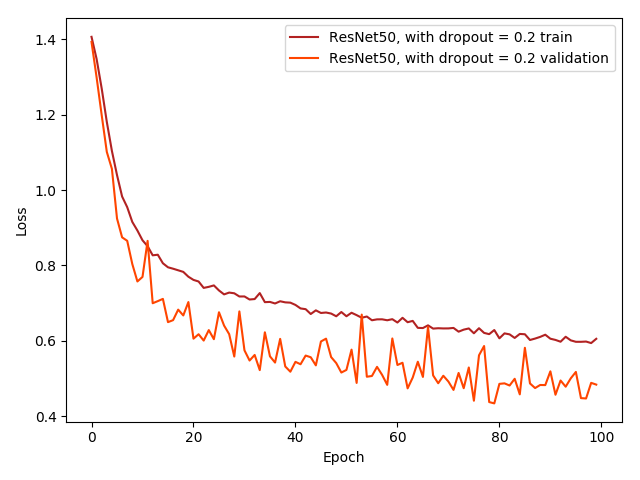
\includegraphics[width = 0.4\textwidth]{plots/resnet50_100e_da02_loss.png}} \\
\end{tabular}
\caption{Performance of ResNet50 with dropout in top model in larger amount of epochs}
\label{fig:resnet50_100e_da02_compare}
\end{figure}

\section{Visualization of first convolutional filters}
In the figure \ref{fig:conv_filters}, first 6 filters from first convolutional block of VGG16 architecture are presented. They extract certain features from images. The first layers are responsible for rather simple features. However, the deeper the layer, the more abstract features it can detect. This is why the base architectures, like VGG16, ResNet50 or InceptionV3 without top layers, already trained on given dataset, are sometimes referred to as 'feature extractors'.
\begin{figure}[!h]
\centering
\begin{tabular}{cc}
	\subfloat{\includegraphics[width = 0.4\textwidth]{../plots/filters/block1_conv1_filter_0.png}} &
	\subfloat{\includegraphics[width = 0.4\textwidth]{../plots/filters/block1_conv1_filter_1.png}} \\
	\subfloat{\includegraphics[width = 0.4\textwidth]{../plots/filters/block1_conv1_filter_2.png}} &
	\subfloat{\includegraphics[width = 0.4\textwidth]{../plots/filters/block1_conv1_filter_3.png}} \\
	\subfloat{\includegraphics[width = 0.4\textwidth]{../plots/filters/block1_conv1_filter_4.png}} &
	\subfloat{\includegraphics[width = 0.4\textwidth]{../plots/filters/block1_conv1_filter_5.png}} \\
\end{tabular}
\caption{First convolutional filters}
\label{fig:conv_filters}
\end{figure}

\newpage
\section{Analysis of predictions}
In the Figure \ref{fig:wrong_predictions} some of wrong predictions of fine-tuned version of VGG16 are shown. Finally, Figure \ref{fig:confusion_matrix} presents the confusion matrix of mentioned network.
\begin{figure}[!h]
\centering
\begin{tabular}{cc}
	\subfloat[Predicted: ostr, true: kękę]{\includegraphics[width = 0.4\textwidth]{wrong_pred/pr_ostr_tr_keke.png}} &
	\subfloat[Predicted: ostr, true: taco]{\includegraphics[width = 0.4\textwidth]{wrong_pred/pr_ostr_tr_taco.png}} \\
	\subfloat[Predicted: otso, true: ostr]{\includegraphics[width = 0.4\textwidth]{wrong_pred/pr_ostr_tr_otso.png}} &
	\subfloat[Predicted: otso, true: taco]{\includegraphics[width = 0.4\textwidth]{wrong_pred/pr_otso_tr_taco.png}} \\
\end{tabular}
\caption{Examples of bad predictions of fine-tuned VGG16}
\label{fig:wrong_predictions}
\end{figure}
\begin{figure}[!h]
\centering
\begin{tabular}{c}
	\subfloat{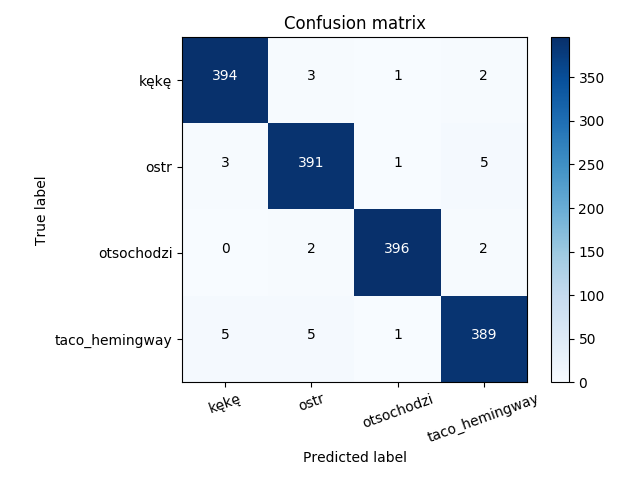
\includegraphics[width = 0.9\textwidth]{plots/confusion_matrix.png}}
\end{tabular}
\caption{Confusion matrix of fine-tuned VGG16}
\label{fig:confusion_matrix}
\end{figure}

\end{document}
